% -------------------------------------------------------------------------------------------------
% Definitionen
% -------------------------------------------------------------------------------------------------
\documentclass[
    fontsize=12pt,                      % Schriftgröße 12 pt
    paper=a4,                           % Seitengröße A4
    twoside=off,                       % zweiseitiger Druck
    DIV=15,                             % Seiteneinteilung
    BCOR=12mm,                          % Bindekorrektur
    headings=normal,                    % normal große Überschriften
    headsepline=false,                   % Trennlinie unter der Kopfzeile
    footsepline=false,                  % Trennlinie über der Fußzeile
    headinclude=true,                   % Kopfzeile zählt zum Textkörper
    footinclude=false,                  % Fußzeile zählt nicht zum Textkörper
    toc=listof,                         % Verzeichnisse der Gleitumgebungen ins Inhaltsverzeichnis
    toc=bib,                            % Literaturverzeichnis ins Inhaltsverzeichnis
    chapterprefix=false,                % vor Kapitelnummern steht "Kapitel"
    appendixprefix=false,               % vor Anhangüberschriften steht "Anhang"
    numbers=noendperiod,                % Keinen Punkt hinter die letzte Zahl eines Kapitels (auch bei Anhang)
    captions=tableabove,                % Tabellenüberschriften setzen
    footnotes=multiple,                 % Erkennung von mehreren Fußnoten hintereinander
    bibliography=oldstyle,              % Literaturverzeichnis: openstyle oder oldstyle
    draft=false,                        % Entwurfsstadium
]{scrreprt}


% Paket Includes
% ----------------------------
\usepackage[T1]{fontenc}                % deutsche Umlaute und Sonderzeichen
\usepackage[utf8]{inputenc}             % Umlaute koennen direkt im Quelltext stehen
\usepackage[ngerman]{babel}             % neue deutsche Rechtschreibung 
\usepackage{lmodern}
\usepackage{graphicx}                   % Bilder einfügen
\usepackage{tabularx}                   % Tabellen mit fester Breite und variabler Spaltenbreite
\usepackage{array,longtable}            % Tabellen mit Seitenumbruch
\usepackage{booktabs}                   % bessere horizontale Linien in Tabellen
\usepackage{array,ragged2e}             % mehr Spaltentypen in Tabellen und neue Spaltentypen
\usepackage{dcolumn}                    % Spalten am Dezimaltrenner ausrichten
\usepackage{amsmath}
\usepackage[                            % Unterabbildungen mit folgenden Parametern:
            font=footnotesize,          % kleine Schrift
            labelfont={sf,bf},          % Labels fett und serifenlos
            textfont={sf},              % Text serifenlos
            format=hang,                % hängender Einzug
           ]{caption}
\usepackage{float}      
\usepackage{hyperref}                   % URL links     
\usepackage{xcolor}  
\usepackage{listings}

\definecolor{mygreen}{rgb}{0,0.6,0}
\definecolor{myred}{rgb}{0.7529,0.3137,0.3019}


\newcommand{\Farbcode}[1]{\texttt{\textbf{\textcolor{myred}{#1}}}}


% Kopf- und Fußzeile
% ----------------------------
\usepackage{scrlayer-scrpage} 
\setkomafont{pagehead}{\sffamily\small}
\setkomafont{pagefoot}{\sffamily\small}
%\automark{chapter}
\lohead{Modul Embedded Systems 2 -- Steuergeräte, Vernetzung, Software} \cohead{} \rohead{Übung 2-3}
\lofoot{\includegraphics[height=10pt]{Figures/HSMW-Logo-klein} HS Mittweida, INW, Prof. Thomanek}
\cofoot{} \rofoot{\thepage}

\pagestyle{headings}
\renewcommand*{\chapterpagestyle}{headings}% Nicht zu empfehlen, aber du willst das offenbar trotzdem.


\setcounter{secnumdepth} {3}
\addto\captionsngerman{\renewcommand{\figurename}{Abb.}}    % Verwende Abb. x.x anstatt Abbildung x.x
\renewcommand{\thefigure}{\arabic{figure}}
% -------------------------------------------------------------------------------------------------
% Dokument
% -------------------------------------------------------------------------------------------------

\begin{document}


\chapter*{Übung 2-3 -- Echtzeitbetriebssysteme}

\section*{FreeRTOS}

In dieser Aufgabe soll das Task-Verhalten aus Übung 2-2 mithilfe des Preemptiven Echtzeitbetriebssystems \textbf{FreeRTOS} umgesetzt werden. Verwenden Sie dafür den Hardwareaufbau aus dem vorherigen Seminar und ergänzen diesen durch einen zusätzlichen Taster am Eingang 2 (siehe Bild).
\begin{figure}[H]
	\centering
	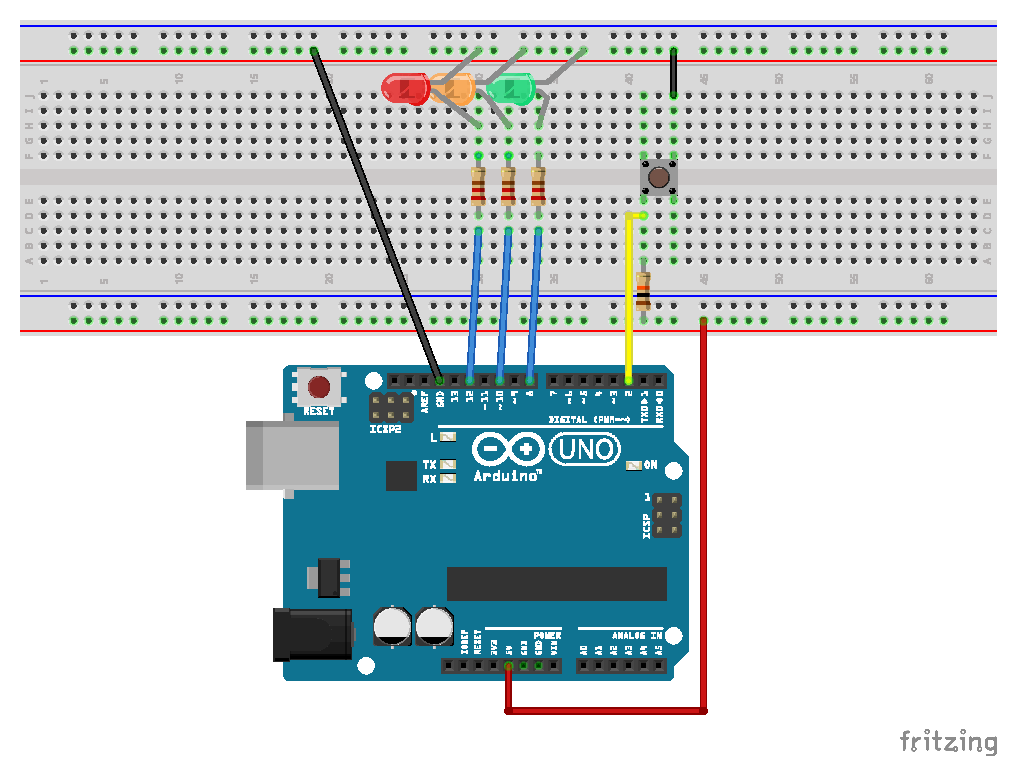
\includegraphics[width=\textwidth]{Figures/Scheduler2_Steckplatine}
\end{figure}
\noindent
In dieser Übung sollen die drei LED -- die jeweils \textbf{durch eine eigene Task} angesteuert werden -- ebenfalls mit unterschiedlicher Frequenz blinken. Zusätzlich soll die Frequenz der LED 1 durch einen Tastendruck verändert werden können. Das \textbf{Überwachen des Tasters} erfolgt über einen Interrupt und \textbf{einer vierten Task}.
\newpage
\noindent
\textbf{Vorbereitungen:}

\begin{itemize}
\item Öffnen Sie den Template-Sketch \Farbcode{FreeRTOSApp.ino} (siehe OPAL)
\item Installieren Sie die FreeRTOS-Bibliothek:
\begin{itemize}
\item Öffnen Sie die Bibliotheksverwaltung unter \texttt{\textbf{Menu $\to$ Bibliothek einbinden $\to$ Bibliothek verwalten...}}
\item Suchen Sie nach \texttt{\textbf{FreeRTOS}}
\item Installieren Sie die Bibliothek \emph{FreeRTOS} von \emph{Phillip Stevens}
\item Sie haben die Bibliothek erfolgreich installiert, wenn das Template-Sketch fehlerfrei übersetzt
\end{itemize}
\end{itemize}

\noindent
\textbf{Implementierung:}

\noindent
\begin{itemize}
\item Erzeugen zu Beginn der \texttt{main}-Funktion eine Queue mit 5 Elementen der Größe 2 Byte (\Farbcode{uint16\_t}) mittels der Funktion \Farbcode{xQueueCreate(...)} (\emph{siehe Seite 3})	
\item Erzeugen im Weiteren vier Tasks:
\begin{itemize}
	\item \Farbcode{Task\_L1} (Prio 2)
	\item \Farbcode{Task\_L2} (Prio 2)
	\item \Farbcode{Task\_L3} (Prio 2)
	\item \Farbcode{Task\_Bt} (Prio 1)
\end{itemize}
mit der Funktion \Farbcode{xTaskCreate(...)} (\emph{siehe Seite 3})
\item Starten Sie am Ende der \texttt{main}-Funktion den Scheduler mittels \\
\Farbcode{vTaskStartScheduler();}
\item Definieren Sie die entsprechenden drei Task-Funktionen für die LEDs, welche in einer Endlosschleife die LED blinken lassen
\item Definieren Sie eine Task-Funktion zum überwachen des Buttons, wobei bei einem erfolgten Tastendruck eine Nachricht (ohne Blockierzeit) in die Queue gelegt werden (Funktion: \Farbcode{xQueueSend(..)} ) (\emph{siehe Seite 3}) -- Dabei soll als Nachricht die \textbf{Intervallzeit} wechselseitig 100 (5 Hz) und 500 (1 Hz) übertragen werden
\item Erweitern Sie die Task der LED 1 um das Lesen aus der Queue (ohne Blockierzeit) mittels der Funktion \Farbcode{xQueueReceive(...)} (\emph{siehe Seite 3}) -- Übernehmen Sie den Wert der Nachricht als neue Intervallzeit für das Blinken der LED

\end{itemize}

\newpage
\noindent
\textbf{Erzeugen einer Task:}
\lstset{language=C++,
	basicstyle=\small\ttfamily,  
	commentstyle=\color{mygreen},
	showstringspaces=false,
	keywordstyle=\color{blue},
	breakatwhitespace=false,        
	breaklines=true}
\begin{lstlisting}[frame=single,  label=LST_MyCam]
BaseType_t xTaskCreate(
             TaskFunction_t pvTaskCode, // z.B. Task_L1
             const char * const pcName, // z.B. "Led 1 blinking"
             uint16_t  usStackDepth, // z.B. 128 (Stacksize)
             void      *pvParameters, // z.B. NULL (no params)
             UBaseType_t uxPriority, // z.B. 2 (Prio)
             TaskHandle_t  *pxCreatedTask ); // z.B. NULL 
                                             // (Task Handle not used)
\end{lstlisting}
\vskip 1cm
\textbf{Erzeugen einer Queue:}
\begin{lstlisting}[frame=single,  label=LST_MyCam]
	QueueHandle_t xQueueCreate( 
	      UBaseType_t uxQueueLength, // z.B. 5 
	      UBaseType_t uxItemSize ); // z.B.  2
\end{lstlisting}

\vskip 1cm
\textbf{Senden einer Nachricht:}
\begin{lstlisting}[frame=single,  label=LST_MyCam]
BaseType_t xQueueSend( 
             QueueHandle_t xQueue,  // myQueue
             const void * pvItemToQueue, // z.B. &data
             TickType_t xTicksToWait ); // 0
\end{lstlisting}

\vskip 1cm
\textbf{Empfangen einer Nachricht:}
\begin{lstlisting}[frame=single,  label=LST_MyCam]
BaseType_t xQueueReceive( 
        	QueueHandle_t xQueue,  // myQueue
        	void * const pvBuffer,
        	TickType_t xTicksToWait ); // 0
\end{lstlisting}



\end{document}